

\documentclass[a4paper]{article}

\usepackage{amsmath}
\usepackage{hyperref}
\usepackage{biblatex}
\usepackage{enumerate}
\usepackage{graphicx}
\usepackage{stmaryrd}
\usepackage[dvipsnames]{xcolor}
\usepackage{listings}
\usepackage{caption}
\usepackage{subcaption}
\usepackage{booktabs}
\usepackage{float}

\addbibresource{refs.bib}

\begin{document}

\author{Ola Bratt \\
  \href{mailto:ola.bratt@gmail.com}{ola.bratt@gmail.com}
  \and
  Patrick Attimont \\
  \href{patrickattimont@gmail.com}{patrickattimont@gmail.com}
}

\title{DAT565/DIT407 Assignment 6}
\date{2024-02-xx}

\maketitle

This paper is addressing the assignment 6 study queries within the \emph{Introduction to Data Science \& AI} course, DIT407 at 
the University of Gothenburg and DAT565 at Chalmers. The main source of information for this project
is derived from the lectures and Skiena~\cite{Skiena:2024}. Assignment 6 is about neural networks.

\section*{Problem 1: The dataset}

The dataset comprises 60,000 training images and 10,000 test images, each measuring 28x28 pixels and in grayscale. 
Every image is associated with a digit label indicating its value. 
Figure \ref{fig:mnist_images} displays a random selection of images from the dataset.



\begin{figure}[H]
  \begin{center}
    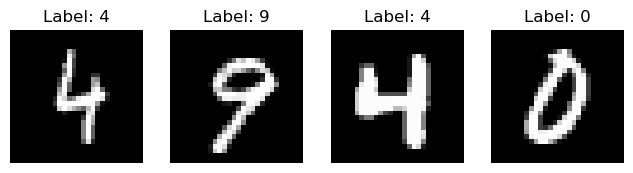
\includegraphics[width=\textwidth]{ola/mnist_images.png}
    \caption{MNIST images}
    \label{fig:mnist_images}
  \end{center}
\end{figure}

\section*{Problem 2: Single hidden layer}

The neural network featuring a single hidden layer encompasses 784 input nodes (28x28), 300 hidden nodes, and 10 output nodes. 
The ReLU function serves as the activation function for the hidden layer, complemented by batch normalization. 
For the output layer, a logarithmic softmax function is utilized since this is a mutliclass problem.
The stochastic gradient descent is used with a learning rate of 0.1.

Tables \ref{tabular:single_hidden_layer_metrics} and Figure \ref{fig:single_hidden_layer} illustrate the metrics for the single hidden layer model. 
The training loss pertains to the loss observed during training, while the test loss represents the loss incurred during testing. 
Test accuracy denotes the accuracy achieved on the test dataset.


\begin{table}
  \begin{center}
  \begin{tabular}{ l|l|l|l }
    \hline
    \text{Epoch} & \text{Training Loss} & \text{Test Loss} & \text{Test Accuracy} \\
    \hline
    1 & 0.2200 & 0.1065 & 0.9695 \\
    2 & 0.1057 & 0.0921 & 0.9725 \\
    3 & 0.0768 & 0.0728 & 0.9765 \\
    4 & 0.0613 & 0.0666 & 0.9793 \\
    5 & 0.0497 & 0.0643 & 0.9791 \\
    6 & 0.0421 & 0.0639 & 0.9798 \\
    7 & 0.0355 & 0.0628 & 0.9811 \\
    8 & 0.0309 & 0.0569 & 0.9823 \\
    9 & 0.0279 & 0.0616 & 0.9796 \\
    10 & 0.0225 & 0.0590 & 0.9816 \\
  \end{tabular}
\end{center}
\caption{Metrics for single hidden layer}
  \label{tabular:single_hidden_layer_metrics}
\end{table}

\begin{figure}[H]
  \begin{center}
    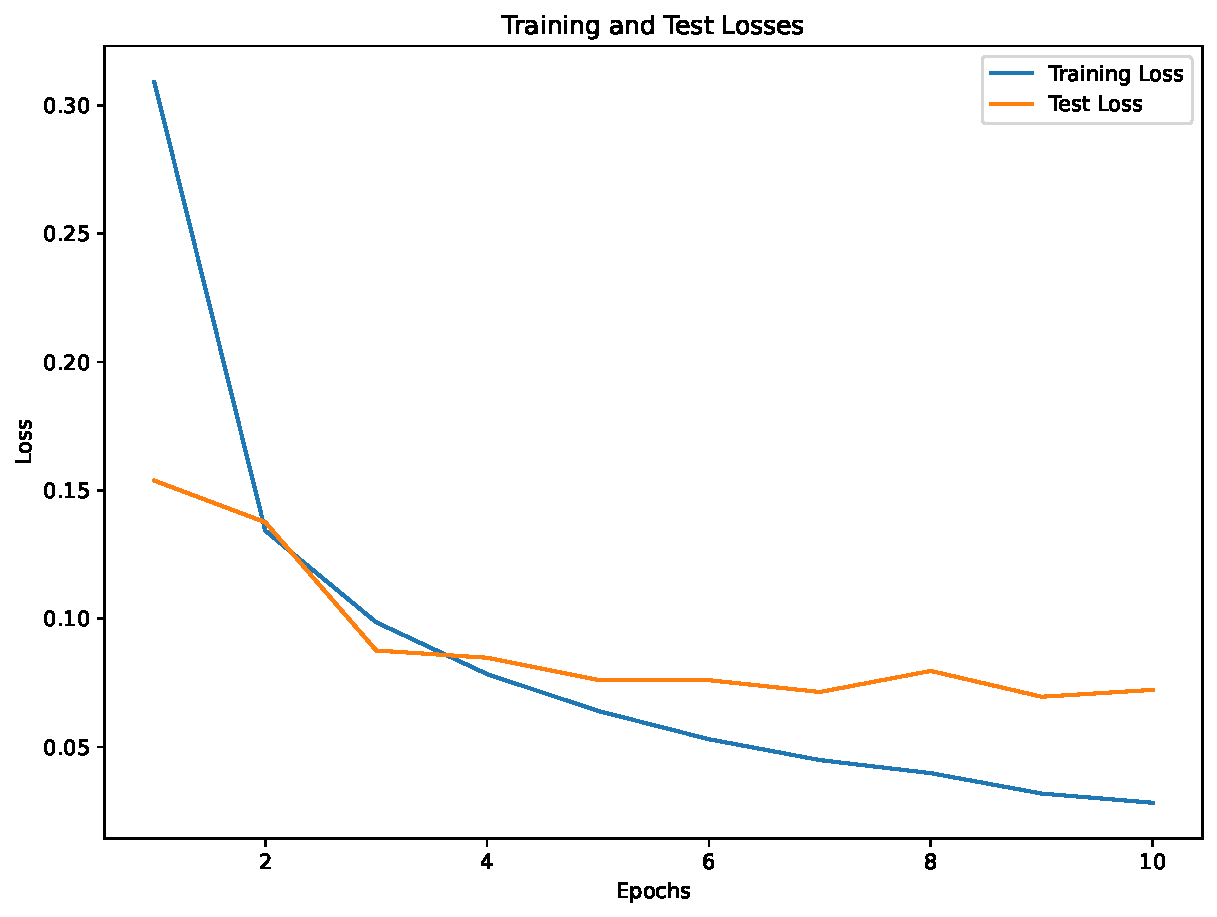
\includegraphics[width=\textwidth]{ola/single_hidden_layer.pdf}
    \caption{Single hidden layer}
    \label{fig:single_hidden_layer}
  \end{center}
\end{figure}

\section*{Problem 3: Two hidden layers}

The neural network with two hidden layers comprises 784 input nodes (28x28), 500 nodes in the first hidden layer, 
300 nodes in the second hidden layer, and 10 output nodes. 
It shares the same layer architecture as the single hidden layer model. 
During training, the optimizer is configured with a weight decay of 0.0001.

Tables \ref{tabular:two_hidden_layers_metrics} and Figure \ref{fig:two_hidden_layers} showcase the metrics for the two hidden layers model.


\begin{table}
  \begin{center}
  \begin{tabular}{ l|l|l|l }
    \hline
    \text{Epoch} & \text{Training Loss} & \text{Test Loss} & \text{Test Accuracy} \\
    \hline
    1 & 0.1935 & 0.0757 & 0.9759 \\
    2 & 0.0892 & 0.0623 & 0.9795 \\
    3 & 0.0633 & 0.0592 & 0.9803 \\
    4 & 0.0477 & 0.0558 & 0.9823 \\
    5 & 0.0390 & 0.0574 & 0.9817 \\
    6 & 0.0319 & 0.0553 & 0.9830 \\
    7 & 0.0262 & 0.0526 & 0.9826 \\
    8 & 0.0226 & 0.0561 & 0.9815 \\
    9 & 0.0199 & 0.0549 & 0.9833 \\
    10 & 0.0175 & 0.0530 & 0.9845 \\
    11 & 0.0176 & 0.0549 & 0.9835 \\
    12 & 0.0136 & 0.0515 & 0.9846 \\
    13 & 0.0120 & 0.0499 & 0.9853 \\
    14 & 0.0111 & 0.0526 & 0.9846 \\
    15 & 0.0122 & 0.0550 & 0.9827 \\
    16 & 0.0103 & 0.0484 & 0.9851 \\
    17 & 0.0097 & 0.0526 & 0.9839 \\
    18 & 0.0082 & 0.0496 & 0.9854 \\
    19 & 0.0086 & 0.0507 & 0.9853 \\
    20 & 0.0073 & 0.0482 & 0.9859 \\
    21 & 0.0091 & 0.0498 & 0.9853 \\
    22 & 0.0083 & 0.0522 & 0.9839 \\
    23 & 0.0095 & 0.0496 & 0.9849 \\
    24 & 0.0086 & 0.0507 & 0.9840 \\
    25 & 0.0080 & 0.0567 & 0.9838 \\
    26 & 0.0065 & 0.0485 & 0.9851 \\
    27 & 0.0069 & 0.0510 & 0.9843 \\
    28 & 0.0073 & 0.0520 & 0.9840 \\
    29 & 0.0069 & 0.0535 & 0.9837 \\
    30 & 0.0056 & 0.0482 & 0.9856 \\
    31 & 0.0061 & 0.0513 & 0.9851 \\
    32 & 0.0068 & 0.0498 & 0.9847 \\
    33 & 0.0047 & 0.0517 & 0.9848 \\
    34 & 0.0058 & 0.0497 & 0.9856 \\
    35 & 0.0072 & 0.0508 & 0.9849 \\
    36 & 0.0075 & 0.0501 & 0.9842 \\
    37 & 0.0061 & 0.0477 & 0.9855 \\
    38 & 0.0063 & 0.0489 & 0.9854 \\
    39 & 0.0052 & 0.0486 & 0.9848 \\
    40 & 0.0058 & 0.0490 & 0.9856 \\
  \end{tabular}
\end{center}
\caption{Metrics for two hidden layers}
  \label{tabular:two_hidden_layers_metrics}
\end{table}



\begin{figure}[H]
  \begin{center}
    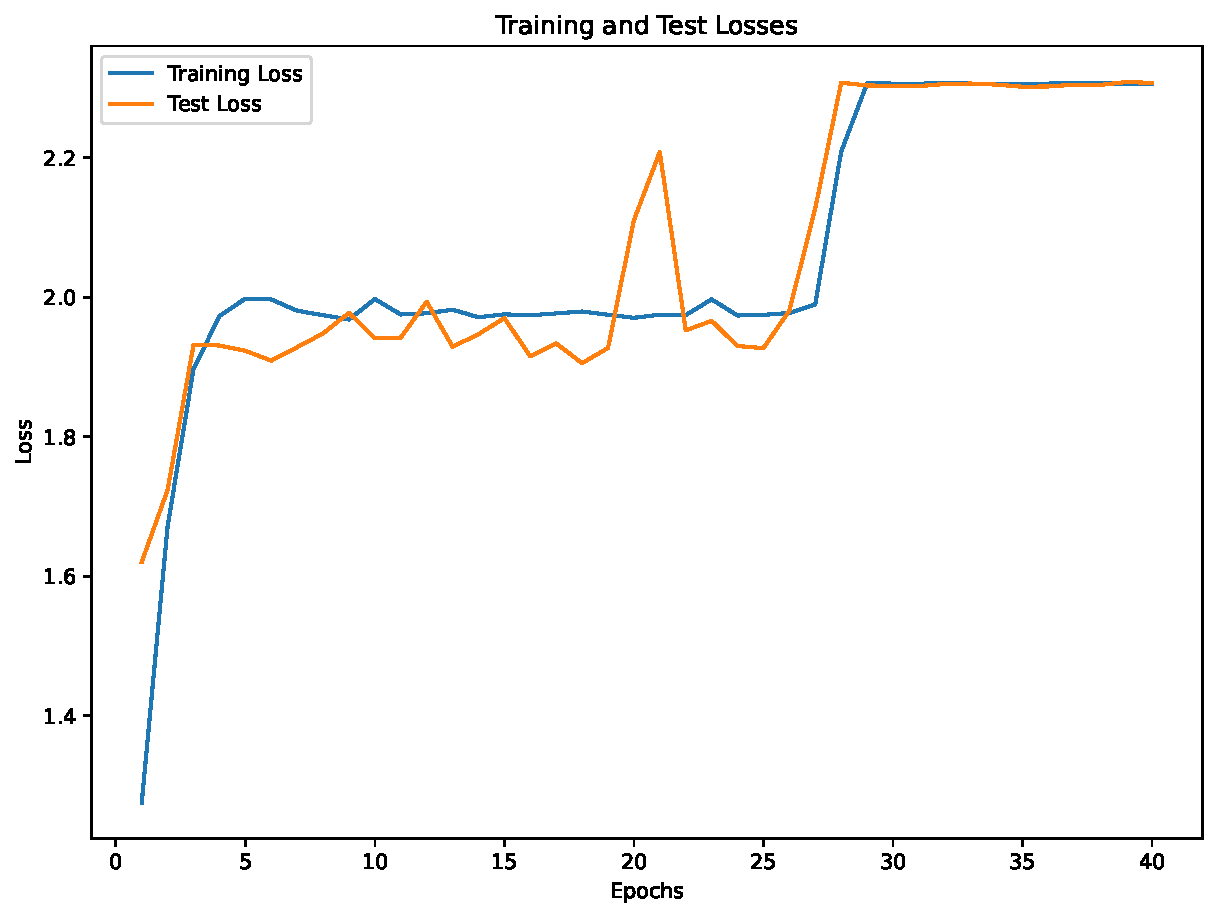
\includegraphics[width=\textwidth]{ola/two_hidden_layer.pdf}
    \caption{Two hidden layers}
    \label{fig:two_hidden_layers}
  \end{center}
\end{figure}

\section*{Problem 4: Convolutional neural network}

The CNN model consists of two convolutional layers, each followed by a max-pooling layer, and two fully connected layers. 
The output layer utilizes logarithmic softmax activation. 
The first convolutional layer has 16 output channels, and the second has 32 output channels.
The fully connected layers have 1568 and 128 neurons, respectively.
The optimization function is a stochastic gradient descent with a learning rate of 0.1 and a weight decay of 0.0001.

Performance metrics for the CNN model trained over 40 epochs are detailed in Tables \ref{tabular:convolutional_neural_network_metrics} and Figure \ref{fig:convolutional_neural_network}

\begin{table}
  \begin{center}
  \begin{tabular}{ l|l|l|l }
    \hline
    \text{Epoch} & \text{Training Loss} & \text{Test Loss} & \text{Test Accuracy} \\
    \hline
    1 & 0.1771 & 0.0477 & 0.9839 \\
    2 & 0.0459 & 0.0328 & 0.9896 \\
    3 & 0.0324 & 0.0306 & 0.9888 \\
    4 & 0.0239 & 0.0334 & 0.9906 \\
    5 & 0.0188 & 0.0275 & 0.9913 \\
    6 & 0.0150 & 0.0276 & 0.9911 \\
    7 & 0.0117 & 0.0275 & 0.9915 \\
    8 & 0.0100 & 0.0277 & 0.9910 \\
    9 & 0.0074 & 0.0253 & 0.9914 \\
    10 & 0.0055 & 0.0303 & 0.9909 \\
    11 & 0.0050 & 0.0270 & 0.9921 \\
    12 & 0.0044 & 0.0316 & 0.9917 \\
    13 & 0.0027 & 0.0297 & 0.9918 \\
    14 & 0.0037 & 0.0278 & 0.9913 \\
    15 & 0.0021 & 0.0263 & 0.9922 \\
    16 & 0.0016 & 0.0268 & 0.9918 \\
    17 & 0.0009 & 0.0262 & 0.9918 \\
    18 & 0.0009 & 0.0246 & 0.9920 \\
    19 & 0.0007 & 0.0256 & 0.9923 \\
    20 & 0.0005 & 0.0263 & 0.9922 \\
    21 & 0.0006 & 0.0254 & 0.9925 \\
    22 & 0.0005 & 0.0245 & 0.9926 \\
    23 & 0.0005 & 0.0251 & 0.9919 \\
    24 & 0.0005 & 0.0244 & 0.9928 \\
    25 & 0.0006 & 0.0248 & 0.9921 \\
    26 & 0.0006 & 0.0259 & 0.9921 \\
    27 & 0.0020 & 0.0257 & 0.9924 \\
    28 & 0.0027 & 0.0268 & 0.9918 \\
    29 & 0.0032 & 0.0371 & 0.9891 \\
    30 & 0.0032 & 0.0275 & 0.9913 \\
    31 & 0.0046 & 0.0283 & 0.9920 \\
    32 & 0.0022 & 0.0298 & 0.9913 \\
    33 & 0.0016 & 0.0273 & 0.9922 \\
    34 & 0.0007 & 0.0318 & 0.9906 \\
    35 & 0.0006 & 0.0257 & 0.9925 \\
    36 & 0.0004 & 0.0256 & 0.9928 \\
    37 & 0.0004 & 0.0258 & 0.9924 \\
    38 & 0.0004 & 0.0252 & 0.9925 \\
    39 & 0.0004 & 0.0247 & 0.9922 \\
    40 & 0.0005 & 0.0249 & 0.9930 \\
  \end{tabular}
\end{center}
\caption{Metrics for Convolutional neural network}
  \label{tabular:convolutional_neural_network_metrics}
\end{table}


\begin{figure}[H]
  \begin{center}
    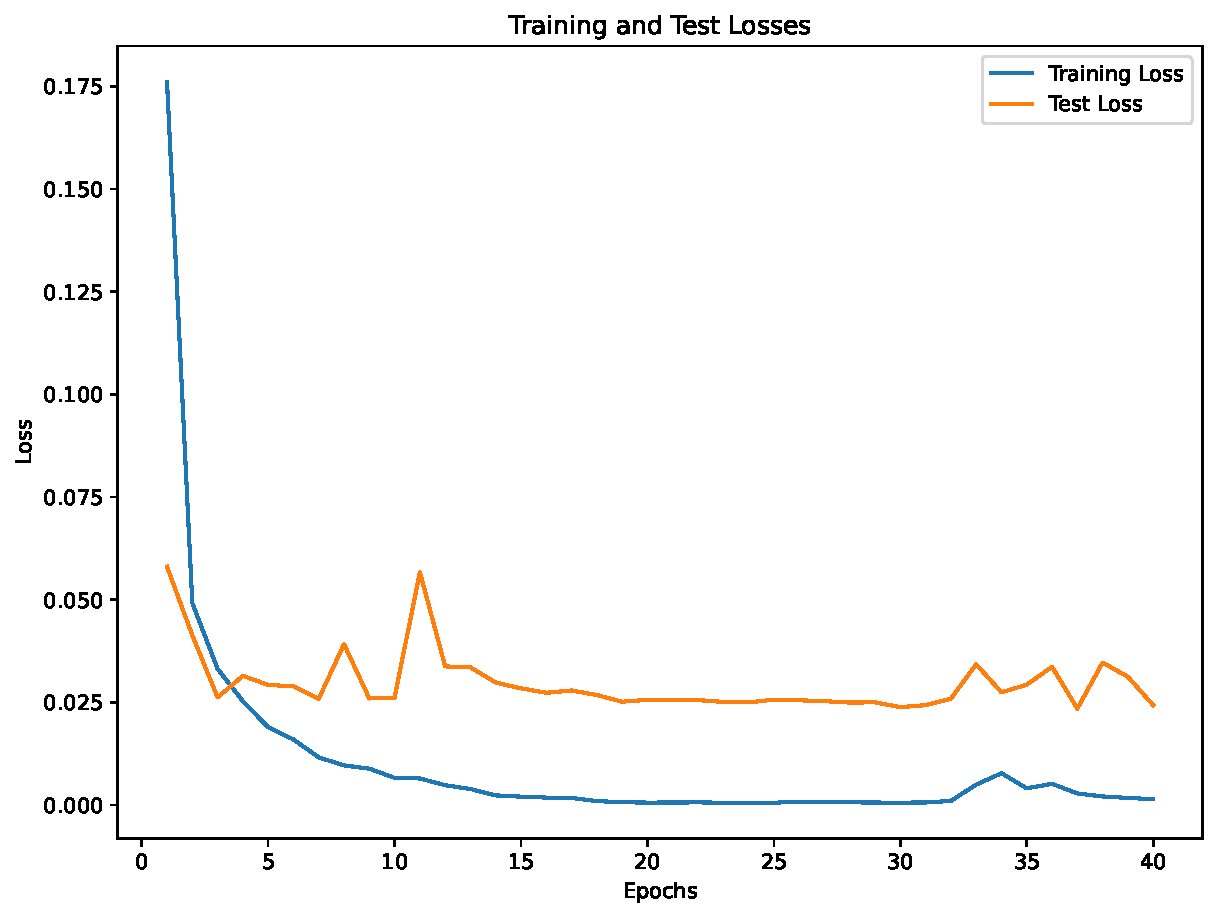
\includegraphics[width=\textwidth]{ola/cnn.pdf}
    \caption{Convolutional neural network}
    \label{fig:convolutional_neural_network}
  \end{center}
\end{figure}


\newpage


\printbibliography

\section*{Appendix: Source Code}

\lstset{
  language=Python,
  basicstyle=\ttfamily,
  commentstyle=\color{OliveGreen},
  keywordstyle=\bfseries\color{Magenta},
  stringstyle=\color{YellowOrange},
  numbers=left,
  basicstyle=\footnotesize,
  breaklines=true,
  postbreak=\mbox{\textcolor{red}{$\hookrightarrow$}\space}
}


\lstinputlisting{ola/assignment6.py}

\end{document}
